% LaTeX Template for Project Report, Version 1.0
% (Abstracted for a Value Education Project Report at NIT Calicut but can be
% modified easily to use for other reports also.)
%
% Released under Creative Commons Attribution license (CC-BY)
%
% Created by: Kartik Singhal
% BTech CSE Batch of 2009-13
% NIT Calicut
% Contact Info: kartiksinghal@gmail.com
%
% It is advisable to learn the basics of LaTeX before using this template.
% A good resource to start with is http://en.wikibooks.org/wiki/LaTeX/
%
% All template fields are marked with a pair of angular brackets e.g. <title here>
% except for the ones defining citation names in ref.tex.
%
% Empty space after chapter/section/subsection titles can be used to insert text.
%
% Just compile this file using pdflatex after making all required changes.

\documentclass[10pt,a4paper]{report}
\usepackage[pdftex]{graphicx} %for embedding images
\usepackage{url} %for proper url entries
\usepackage{float}
\usepackage[dvips, bookmarks, colorlinks=false, pdfborder={0 0 0}, pdftitle={NoSQL}, pdfauthor={Shubhangam Agrawal}, pdfsubject={NoSQL}, pdfkeywords={Databases, Cloud Computing, Big Data}]{hyperref} %for creating links in the pdf version and other additional pdf attributes, no effect on the printed document
%Prevent Hyphenation
%\usepackage[none]{hyphenat}
%\raggedright

\begin{document}
\renewcommand\bibname{References} %Renames "Bibliography" to "References" on ref page

%include other pages
\begin{titlepage}

\begin{center}

\textup{\large Major Project Mid--Term Evaluation report on}\\[1.0cm]

% Title
\uppercase{\Large \textbf {Extraction and classification of questions from the Internet using a Machine Learning approach.}}\\[3.0cm]

% Done by
\normalsize Done by \\
\begin{table}[h]
\centering
\begin{tabular}{lr}\hline \\
Alok Saw & B090924CS \\ 
Jerrin Shaji George & B090437CS \\ 
Shubhangam Agrawal & B090904CS \\ 
Stein Astor Fernandez & B090006CS \\ \\ \hline 

\end{tabular}
\end{table}

\normalsize Guided by \\ 
\begin{table}[h]
\centering
\begin{tabular}{lr}\hline \\
Dr. Priya Chandran \\ \\ \hline

\end{tabular}
\end{table}

\vfill

% Bottom of the page

\includegraphics[width=0.20\textwidth]{./nitc-logo}\\[1cm]
\LARGE{Department of Computer Science and Engineering}\\
\normalsize
\textsc{National Institute of Technology Calicut}\\
Calicut, Kerala 673 601 \\
\vspace{0.5cm}
Monsoon Semester 2012

\end{center}

\end{titlepage}

\newpage
\thispagestyle{empty}

\begin{center}

\huge{Computer Science and Engineering}\\
\normalsize
\textsc{National Institute of Technology Calicut}\\[2.0cm]

\emph{\LARGE Certificate}\\[2.5cm]
\end{center}
\normalsize This is to certify that this is a bonafide report for the mid--term evaluation presented by \textbf{Alok Saw, Jerrin Shaji George, Shubhangam Agrawal and Stein Astor Fernandez} during Monsoon Semester 2012 in partial fulfilment of the requirement of the Major Project I.\\[1.0cm]

\vfill

% Bottom of the page
\begin{flushright}
Faculty In-charge\\[1.5cm]
Course Co-ordinator\\[1.0cm]
\end{flushright}

\begin{flushleft}
Date:
\end{flushleft}

\vspace{2in}
\begin{abstract}

Today, there is a massive amount of data available on the internet. While search engines have made searching for relevant pages trivial, extracting only the relevant sections of data from the huge set of search results has become very important. A machine learning approach to tackle this problem has the capability to keep adapting to the rapidly changing dynamics of the internet.

We plan to make an application which will take a topic as input and return a list of questions based on the topic from the internet and classify them based on difficulty.

The application will use popular web search engines to generate a list of pages which may contain questions pertaining to the supplied topic. Each page will be parsed into sections, each of which will then be analyzed using a machine learning approach to decide whether it is a relevant question or not and assign it a difficulty classification. 


\end{abstract} 


\pagenumbering{roman} %numbering before main content starts
\tableofcontents

\newpage
\pagenumbering{arabic} %reset numbering to normal for the main content

\chapter{Literature Survey}

We searched for various papers related to machine learning, classification and labelling of text sections related to a topic. Considering as this is a field with a lot of ongoing research and work, we found a fair few number of published papers which we read to gain an insight into the approach that we will follow.\\

Teevan et al.\cite{teevan} have discussed the relevance of using search methodologies that focus more on contextual information as opposed to simple keyword matching as that may not be enough the capture the relevant text. 

Joachims has also concluded\cite{joachims} that SVMs are an effective text classification tool which uses the Supervised Machine Learning model. 

Inoue et al.\cite{squint} proposes an SVM based approach to identify the most relevant section in Web pages returned by a search query (SQUINT) and provides an architectural overview of the same. To accomplish this it uses a feature set generated by the Supervised Learning model. \\

We explore a similar architecture to SQUINT in order to have a machine learning approach to extracting questions based on topics from web pages.

\chapter{Design}

We have settled on a component---based architecture for the application which we believe will be feasible to implement. 

Having a component based architecture is suitable for this application because each component has a well defined function which is more-or-less independent of the other sections. 
This will help in having a de-coupled structure and each component can be modified without affecting the other components. 

\section{Components}

The high---level view of the architecture is as follows : 

\begin{center}
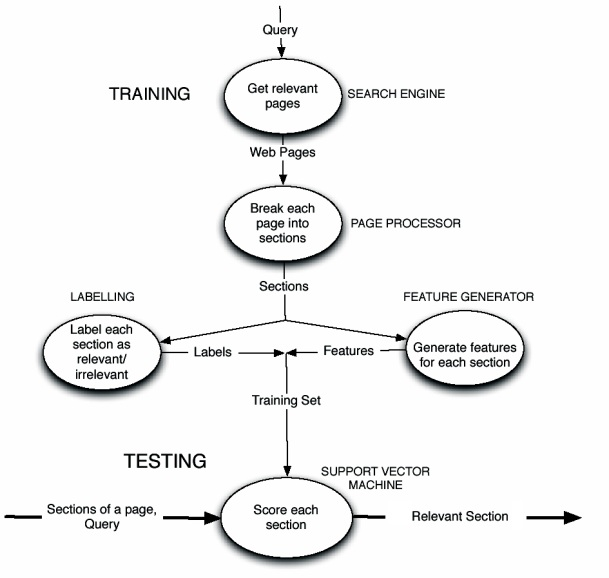
\includegraphics[width=0.80\textwidth]{./architecture}\\
\end{center}

\subsection{Query}

Firstly, we will take the input of the topic and generate a list of sub-topics and other keywords which relate to the topic. For eg. if the topic is ``Operating Systems", various sub-topics can be ``Processes", ``Threads", "Memory Management" etc.

This list of keywords will then be used to generate a number of key--phrases comprising set Q which will be queried on the search engine to get a list of pages which are likely to contain questions related to the required topic. These pages will comprise the set P.

\subsection{Page Preprocessor}

Each page that we load will need to be stripped of all useless markup data, links and pictures and we need to parse out only the text portions available on the page which may contain the questions. 

The page will then be broken into various sections which will be passed onto the further components.

The set S will contain all sections from all pages that we have loaded: 

\textit{S = \{s; s is a section in some page in P\}}

\subsection{Feature Generator}

The feature generator will generate the features and statistics for each section, which will be analysed by the SVM to create the regression model, based on the following : 

\begin{itemize}
	\item Word Rank Based Features
	\item Bigram Rank Based Features
	\item Coverage of Top Ranked Tokens
	\item Distance from the Query
	\item Query Word Frequency
\end{itemize}

\subsection{Labelling}

For generating the training set, we will manually label a set of sections as to whether they are relevant questions of the given topic or not and this data will be used by the SVM to generate the model. The difficulty level of the question will also be given a rating on a scale of 10.

\subsection{Support Vector Machine}

The Support Vector Machine component will be trained using the Training Set comprising of the section set with the generated features and manually tagged labels. 

This will use the data to generate a regression model. \\

This will then be used to identify the relevant questions sections and will also assign them a difficulty rating. \\

The SVM based approach to identify the most relevant section in a web--page (SQUINT) \cite{squint} was developed to deal with big sections of text but can be adapted to our use--case by tweaking the feature-set parameters. 

\subsection{Output}

The output component will take all the questions extracted and output them in a clean format sorted on the basis of difficulty.

\section{Programming Language}

With regards to programming language in which we will implement the project, we have narrowed down the choices to the following : 
\begin{description}
	\item[Java] A very popular Object Oriented Language with lots of packages available for most algorithms and data structures.
	\item[Octave] An interpreted language with support for Machine Learning models.
\end{description}

\chapter{Further Work}

While the overall architecture of the application seems promising, each component needs to be designed with an elaborate algorithm and appropriate data structures need to be chosen after detailed analysis. \\

We will continue to follow the latest research related to machine learning in order to tune the machine learning algorithm which will identify questions. \\

Once the design is finalised, we plan to start the basic implementation of the application and hope to achieve significant progress on at least 1 component by the end of this semester.


\clearpage
\addcontentsline{toc}{chapter}{References}
\begin{thebibliography}{99}

\bibitem{teevan} The Perfect Search Engine is Not Enough : A Study of Orienteering Behavior in Directed Search, \textbf{Jaime Teevan, Christine Alvarado, Mark S. Ackerman and David R. Karger}, \textit{Proceedings of the SIGCHI conference on Human factors in computing systems. pp. 415-422, April 2004.}

\bibitem{joachims} Text Categorization with Support Vector Machines: Learning with Many Relevant Features, \textbf{Thorsten Joachims}, \textit{Universitat Dortmund, Informatik LS8, Baroper Str. 301, 44421 Dortmund, Germany}

\bibitem{squint} SQUINT � SVM for Identification of Relevant Sections in Web Pages for Web Search, \textbf{Riku Inoue, Siddharth Jonathan J.B., Jyotika Prasad}, \textit{Department of Computer Science, Stanford University}

\bibitem{wiki} Machine Learning, \ \url{http://en.wikipedia.org/wiki/Machine_Learning}

\bibitem{coursera} Machine Learning Course on Coursera, \ \url{https://class.coursera.org/ml-2012-002/class/index}

\end{thebibliography}


\end{document}
